\documentclass[aspectratio=169,10pt]{beamer}
%\documentclass[10pt]{beamer}

%\documentclass[7pt]{beamer}
%\usepackage[size=custom,width=16,height=9,scale=1]{beamerposter}
\usetheme{Ruco}
\usepackage[utf8]{inputenc}  
\usepackage[T1]{fontenc}    
\usepackage[spanish]{babel}
\usepackage{amsmath,amsfonts,amsbsy}
\usepackage{xcolor}
\usepackage{graphicx}
\usepackage{animate}
\usepackage{float}
\usepackage{ifthen}
\usepackage{tabularray}
\usepackage{booktabs}
\UseTblrLibrary{booktabs}
\usepackage{tikz}
\usetikzlibrary{positioning,calc,arrows, arrows.meta,tikzmark}
\usepackage{multicol}
\usepackage{multirow}

\title{Sistema de Seguridad en Laboratorio:}
\subtitle{Interfaz gráfica en LabVIEW con implementación de APIs como AWS y Google Cloud}
\author{Daniel Alejandro Martínez Lara}
\institute{IICO-UASLP}
\date{1 de junio de 2026}
\newcommand{\gifon}{1}

\begin{document}

\begin{frame}
\titlepage
\end{frame}
\begin{frame}[t]{Contenido}{}
     \begin{multicols}{2}
     \tableofcontents
     \end{multicols}
     \end{frame}
 
% \AtBeginSection[]{
%     \begin{frame}<beamer>
%         \frametitle{Contenido}
%         \begin{columns}[T]
%             \begin{column}{.5\textwidth}
%                 \tableofcontents[currentsection,sections=1-2]
%             \end{column}
%             \begin{column}{.5\textwidth}
%                 \tableofcontents[currentsection,sections=3-5]
%             \end{column}
%         \end{columns}
%     \end{frame}
% }

\section{Introducci\'on}

\begin{frame}[t]{Introducción}{Definiendo el problema.}
    \begin{tikzpicture}[remember picture,overlay]
        \node[anchor=center,text width=16cm, scale=.9, align=justify,yshift=-3cm] (text1) at (current page.north){
            Durante el desarrollo de la materia de LabVIEW se toco el tema acerca de la implementación de APIs en el programa, facilitando procesos de reconocimiento de imagenes ya que primeramente empezamos con el sistema VISION integrado en LabVIEW, pero con la limitancia de lo impresiso que podia ser el programa.
            \\
            Con esta migración a un nuevo sistema de reconocimiento es que comenzo un interes por estos sistemas.
            \\
            Ya que esta aplicación trata del trabajo en la curiosidad de como podia implementarse a un sistema de seguridad.
        };

        \node[anchor=center,scale=.08,xshift=-50cm,yshift=-25cm](lblogo) at (text1.south){
\includegraphics{images/title-page/labviewlogo.jpeg}};
        
        \node[anchor=center,scale=.03,xshift=0cm,yshift=-30cm](AWS) at (text1.south){
\includegraphics{images/title-page/Amazon-Web-Services-AWS-Logo.png}};
        
        \node[anchor=center,scale=.4,xshift=12cm,yshift=-5cm](googlesv) at (text1.south){
\includegraphics{images/title-page/Google-Cloud-Logo-PNG-Pic.png}};
    \end{tikzpicture}
\end{frame}

\section{Objetivos}

\begin{frame}[t]{Objetivos}{Problemas a solucionar}
    \begin{tikzpicture}[remember picture,overlay]
        \node[anchor=center,text width=16cm,scale=.9,align=justify,yshift=3cm](tx1) at (current page.center){
            Para este proyecto tenemos los siguientes objetivos a cumplir durante el desarrollo del programa:
        };
        \node[anchor=center,text width=8cm,scale=.9,align=justify,yshift=-2.5cm,xshift=4cm](tx2) at (tx1.south west){           
            \begin{itemize}
                \item implementación de escaneo de código QR para el programa.
                \item Verificación de existencia del usuario dentro de una base de datos basada en Google Sheets.
                \item Verificación de equipo de seguridad del usuario para autorizar su acceso.
                \item Registro de cada intento de acceso y cada acceso autorizado por parte de los usuarios.
            \end{itemize}};
        
        \node[anchor=center,scale=.15,xshift=25cm,yshift=-4cm] (lab1) at (tx2.east){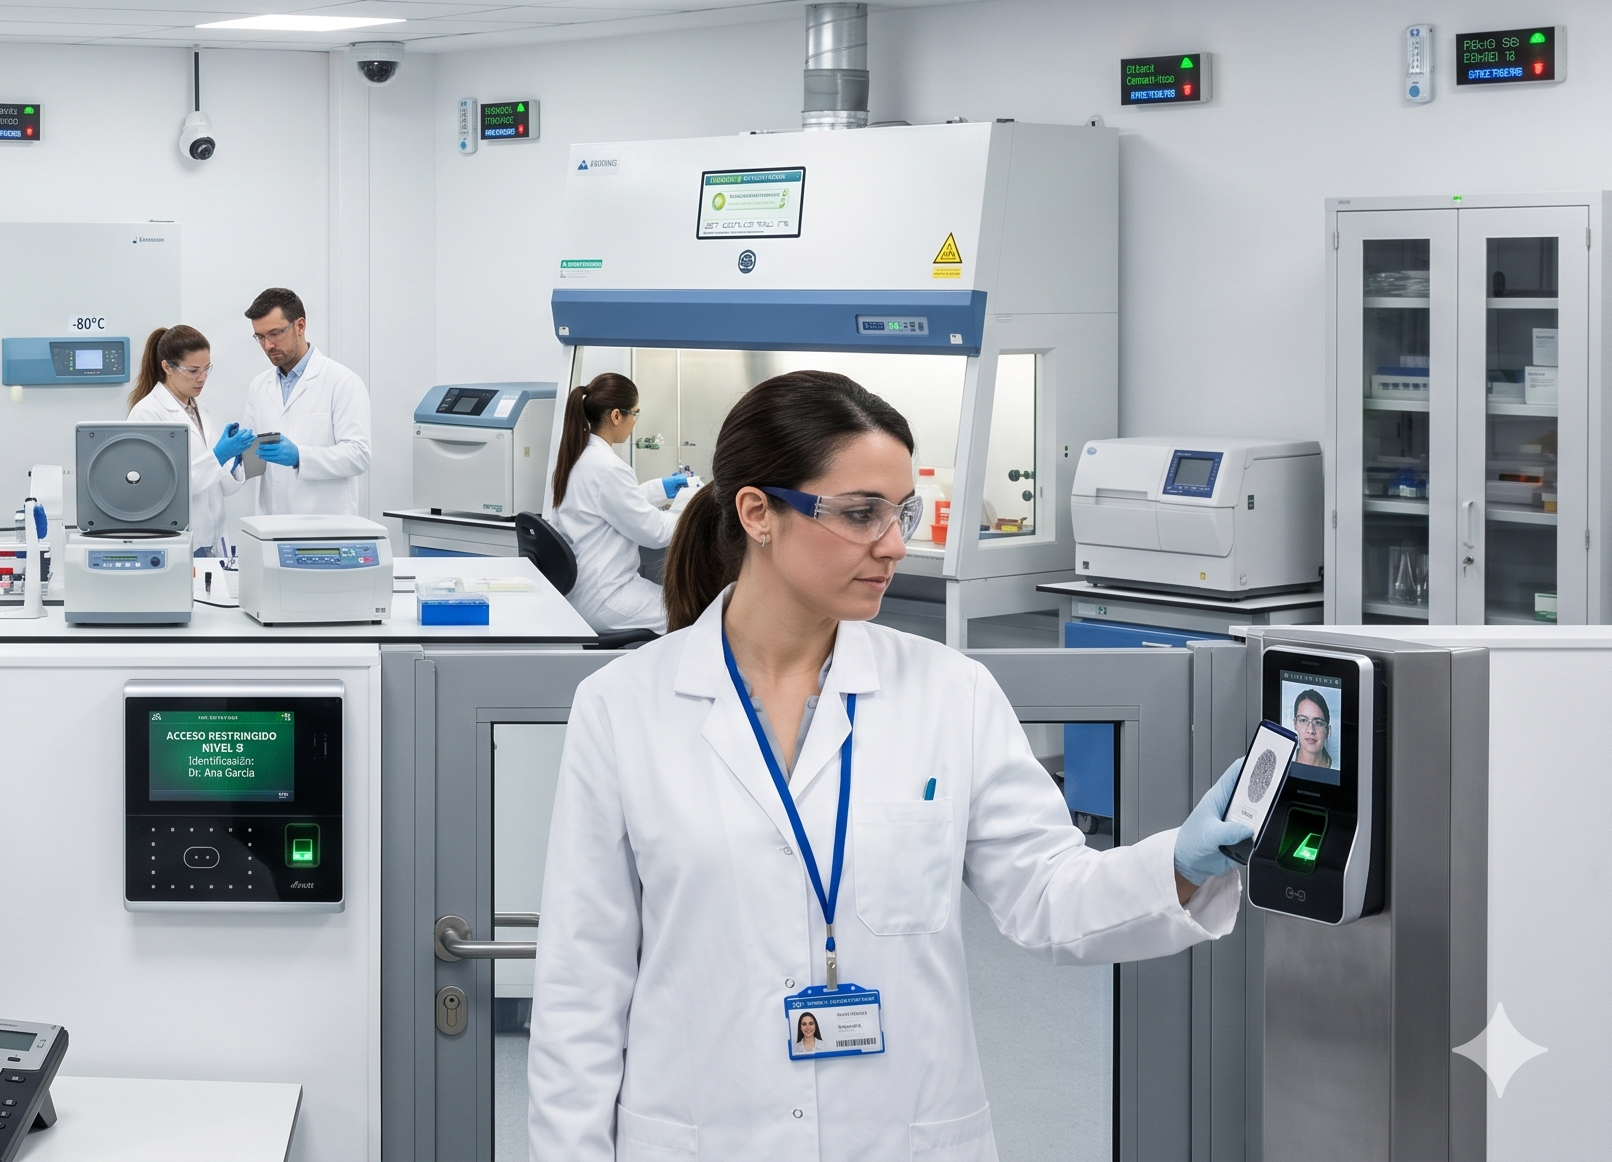
\includegraphics{images/title-page/labo1.png}};

    \end{tikzpicture}
\end{frame}
\section{Desarollo del Programa}

\subsection{Programas de Python (Reconocimiento de usuario)}

\begin{frame}[t]{Programas de Python}{Reconocimiento de Usuario (Google Services)}
    \begin{tikzpicture}[remember picture,overlay]
        \node[anchor=center,scale=.9,text width=16cm,align=justify,xshift=0cm,yshift=2.8cm](tx1) at (current page.center){
            Como primer programa implementado se realizo un programa en python con comuncación de una API desarrollada por Google Services, con la ayuda de la libreria \textbf{gspread} es que se logra esta comunicación. 
        };

        \node[anchor=center,scale=.32,xshift=9cm,yshift=-9cm] (im1) at (tx1.south west){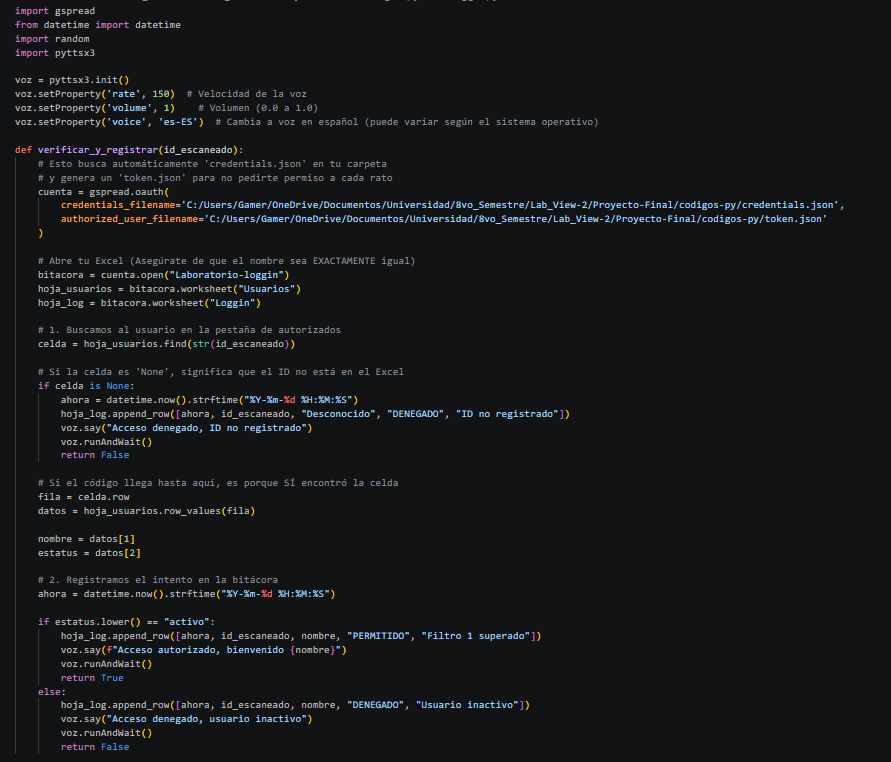
\includegraphics{images/title-page/logincode1.png}};

        \node[anchor=center,scale=.18,xshift=59cm,yshift=-16cm] (im2) at (tx1.south west){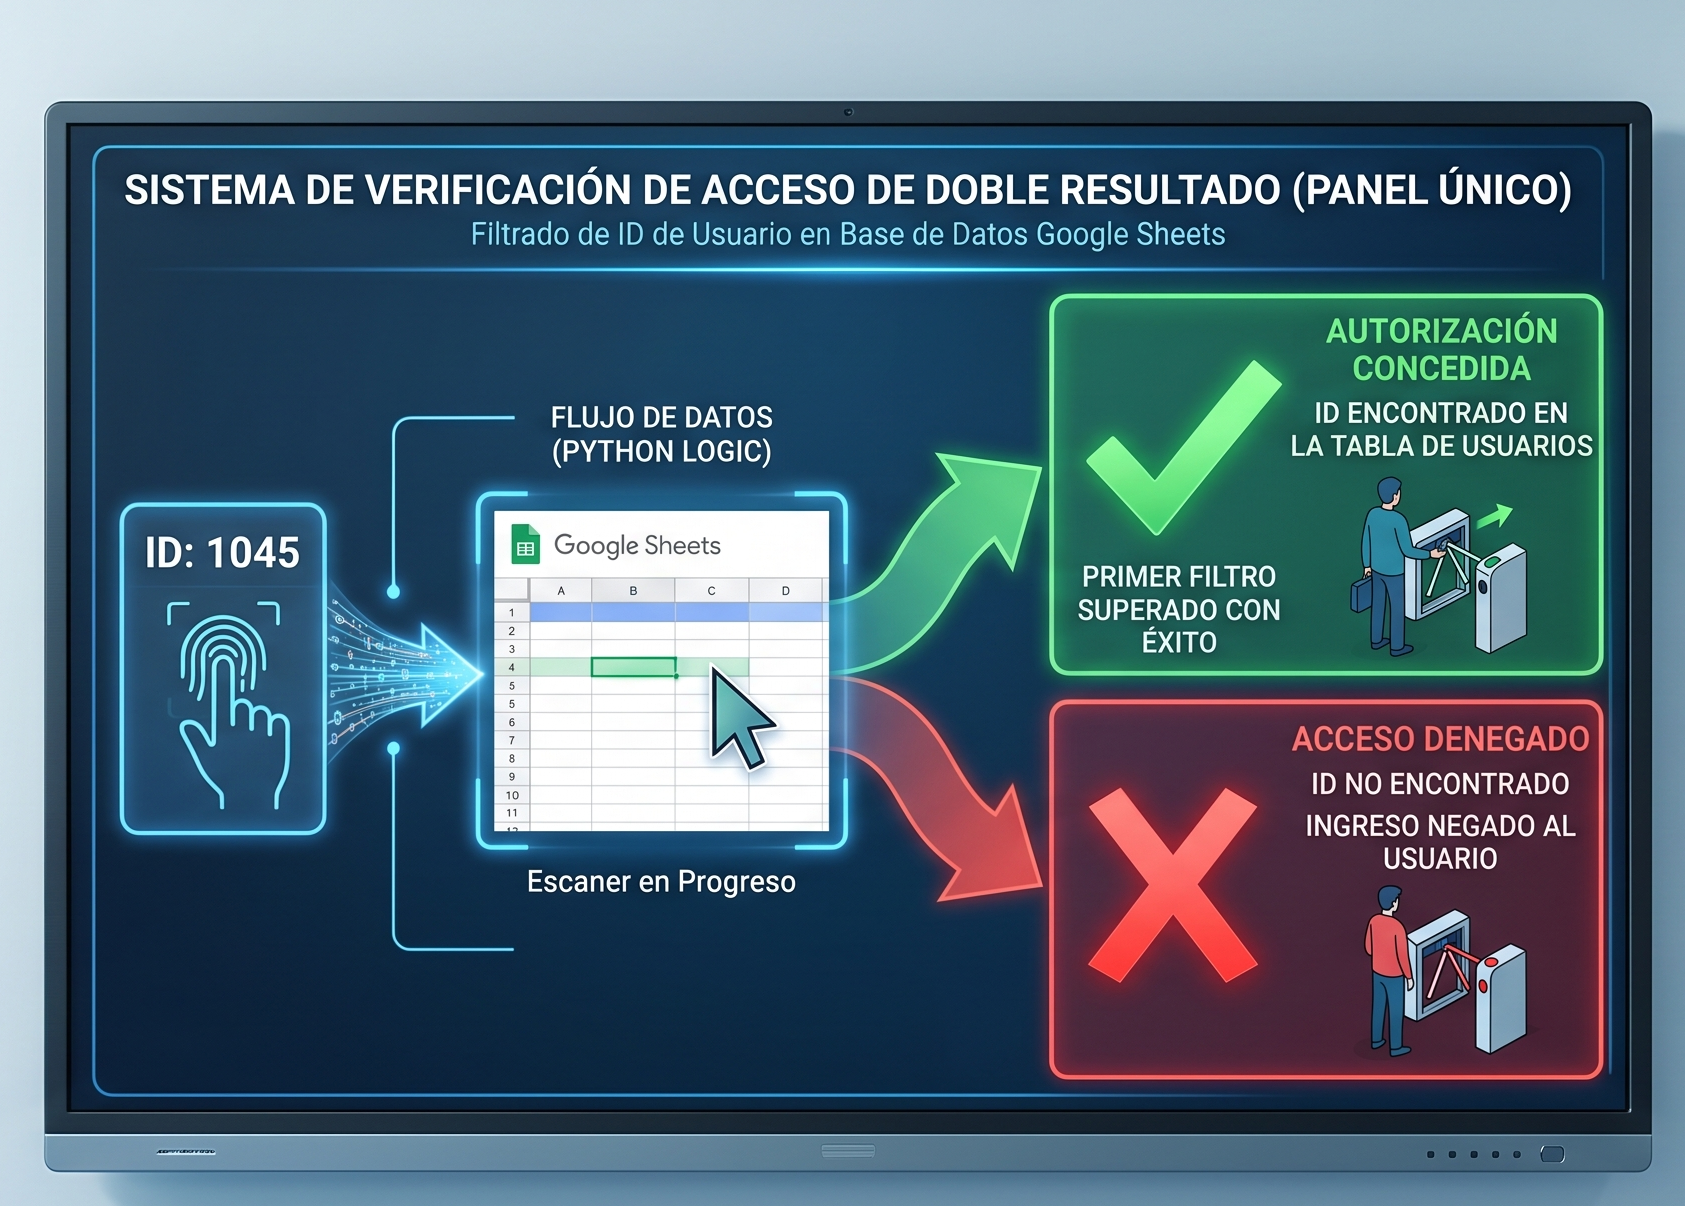
\includegraphics{images/title-page/coderepresent1.png}};
        
        
    \end{tikzpicture}
\end{frame}

\subsection{Programas de Python (Reconocimiento de equipo)}

\begin{frame}[t]{Programas de Python}{Reconocimiento de equipo de Laboratorio (AWS)}
    \begin{tikzpicture}[remember picture,overlay]
        \node[anchor=center,scale=.9,text width=16cm,align=justify,xshift=0cm,yshift=2.8cm](tx2) at (current page.center){
            Como segundo programa implementado se realizo un programa en python con comuncación de una API desarrollada por Amazon Web Services (AWS), con la ayuda de la libreria \textbf{boto3} es que se logra esta comunicación. 
        };

        \node[anchor=center,scale=.32,xshift=8cm,yshift=-9cm] (im3) at (tx2.south west){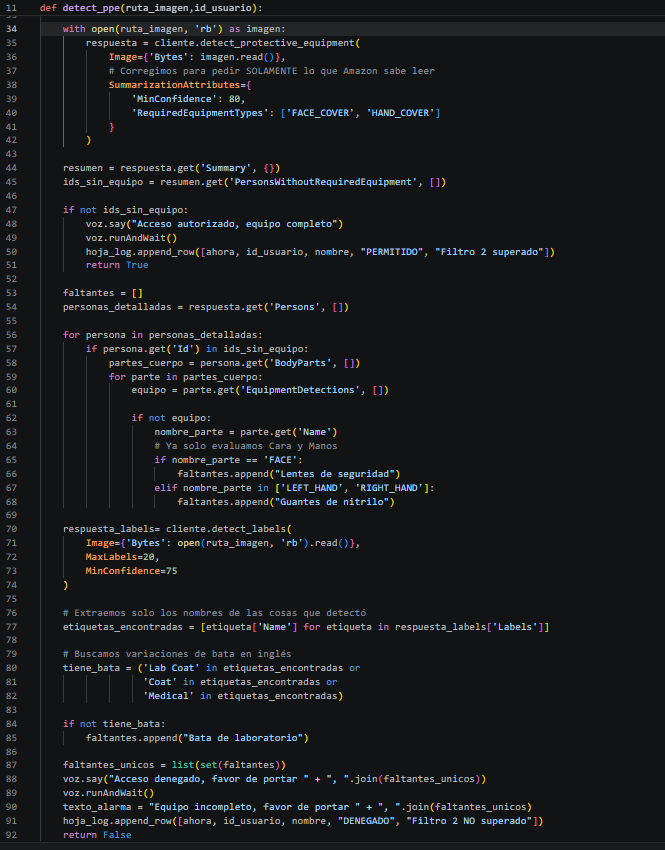
\includegraphics{images/title-page/logincode2.png}};

        \node[anchor=center,scale=.09,xshift=110cm,yshift=-30cm] (im4) at (tx2.south west){\includegraphics{images/title-page/coderepresent2.png}};

    \end{tikzpicture}
\end{frame}

\subsection{Interfaz de LabVIEW (Conexión con Python)}

\begin{frame}[t]{Interfaz de LabVIEW}{Conexión con Python}
    \begin{tikzpicture}[remember picture,overlay]
        \node[anchor=center,scale=.9,text width=16cm,xshift=0cm,yshift=3cm,align=justify] (tx3) at (current page.center){
            Para conectar LabVIEW con Python se utilizo la siguiente funcion dentro de LabVIEW:
            \\
            \textbf{Python NODE:} Esta función se encarga de ejecutar el archivo de Python y obtener el dato de salida para poder trabajarlo dentro de LabVIEW.
        };

        \node[anchor=center,scale=.7,xshift=0cm,yshift=-5cm] (im5) at (tx3.south){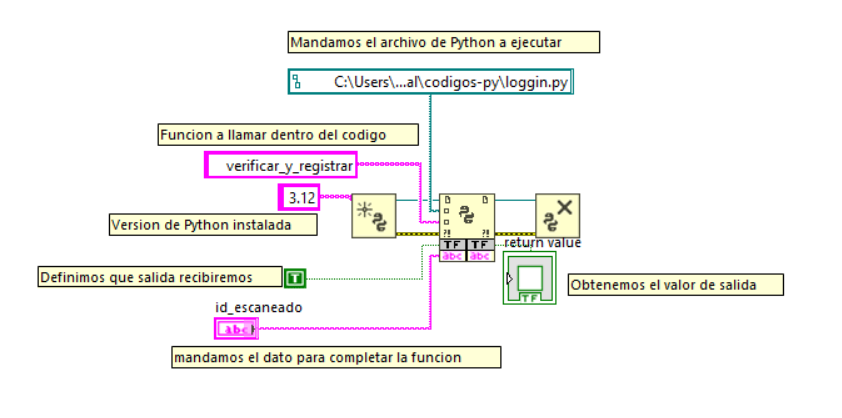
\includegraphics{images/title-page/lb-con1.png}};
        
    \end{tikzpicture}
    
\end{frame}

\subsection{Programa en LabVIEW pt.1}

\begin{frame}[t]{Interfaz en LabVIEW}{Diagrama de flujo pt.1}
    \begin{tikzpicture}[remember picture,overlay]
        \node[anchor=center,scale=.9,text width=16cm,xshift=0cm,yshift=3.5cm,align=justify] (tx4) at (current page.center){
            La implementación del programa dentro del entorno de LabVIEW fue de la suguiente forma.
        };

        \node[anchor=center,scale=.65,xshift=0cm,yshift=-5.5cm] (im6) at (tx4.south){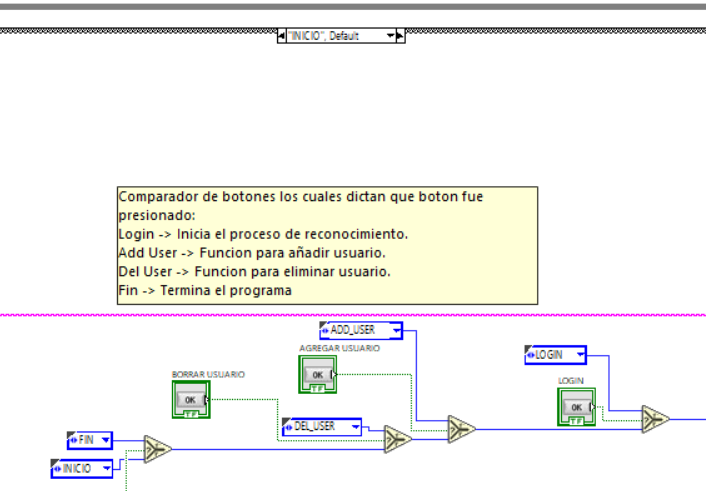
\includegraphics{images/title-page/lb-con2.png}};
    \end{tikzpicture}
\end{frame}

\subsection{Programa en LabVIEW pt.2}

\begin{frame}[t]{Interfaz en LabVIEW}{Diagrama de flujo pt.2}
    \begin{tikzpicture}[remember picture,overlay]
        
        \node[anchor=center,scale=.45,xshift=-9.5cm,yshift=-1cm] (im8) at (current page.east){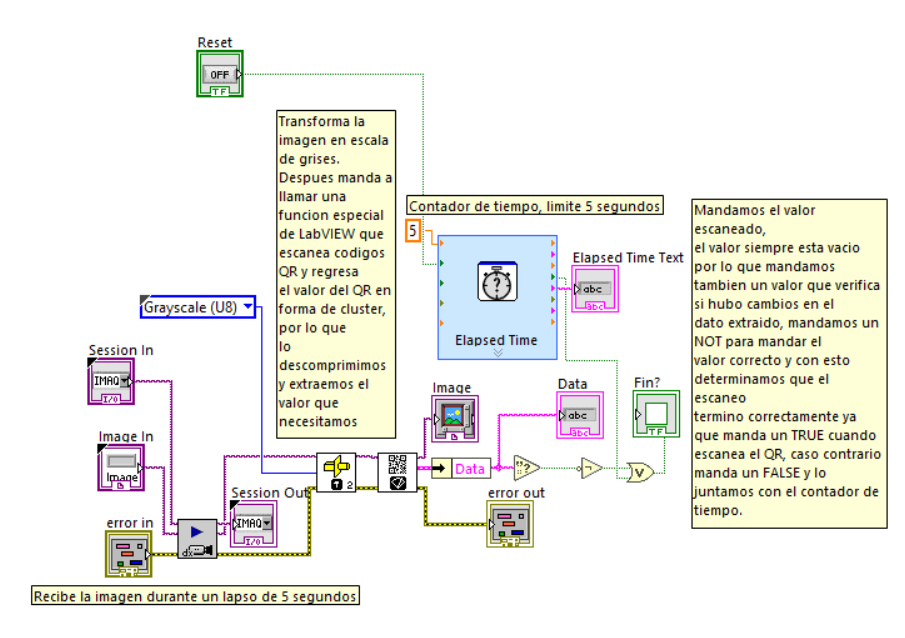
\includegraphics{images/title-page/lb-con4.png}};
        
        \node[anchor=center,scale=.9,text width=8cm,xshift=2cm,yshift=0cm,align=justify] (tx5) at (im8.north){
            Dentro del subVI que escanea el QR\dots
        };

        \node[anchor=center,scale=.5,xshift=8cm,yshift=0.5cm](im7) at (current page.west){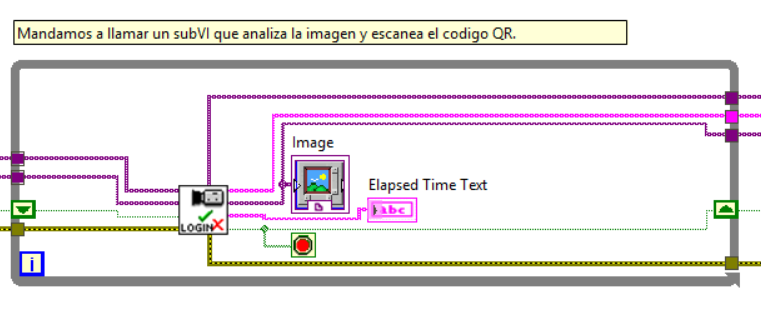
\includegraphics{images/title-page/lb-con3.png}};

        \node[anchor=center,scale=.9,text width=8cm,xshift=2cm,yshift=0cm,align=justify] (tx6) at (im7.north){
            Primer análisis que nos recibe\dots
        };

    \end{tikzpicture}
\end{frame}

\subsection{Programa en LabVIEW pt.3}

\begin{frame}[t]{Interfaz en LabVIEW}{Diagrama de flujo pt.3}
    \begin{tikzpicture}[remember picture,overlay]

        \node[anchor=center,scale=.35,xshift=-12cm,yshift=0cm] (im9) at (current page.east){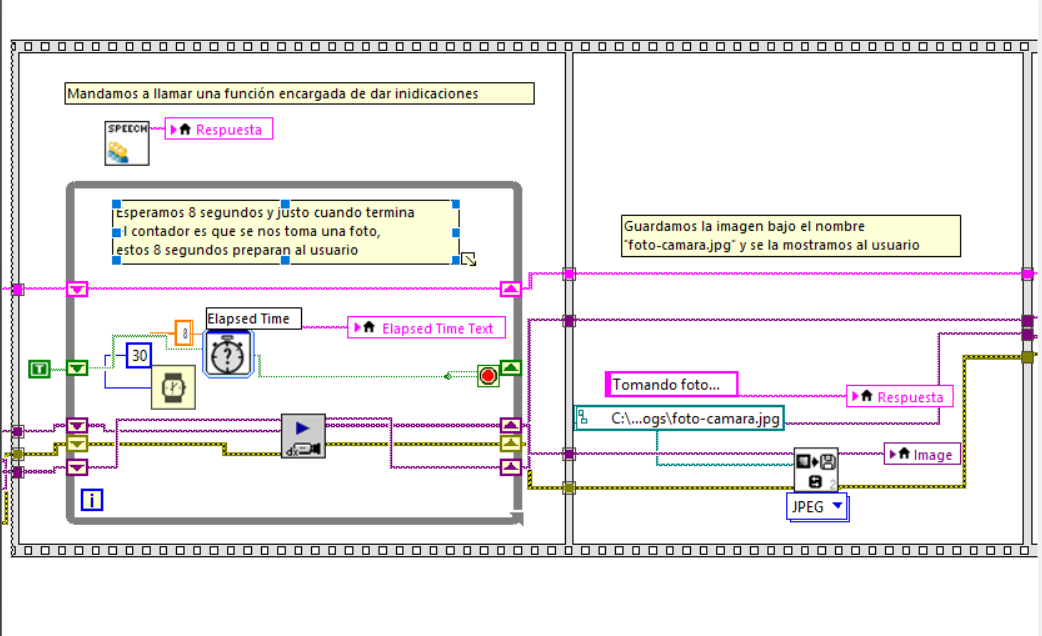
\includegraphics{images/title-page/lb-con6.png}};
        
        \node[anchor=center,scale=.9,text width=8cm,xshift=2cm,yshift=0cm,align=justify] (tx7) at (im9.north){
            Si la persona pasa el 1er filtro\dots    
        
        };

        \node[anchor=center,scale=.35,xshift=11cm,yshift=0.5cm](im10) at (current page.west){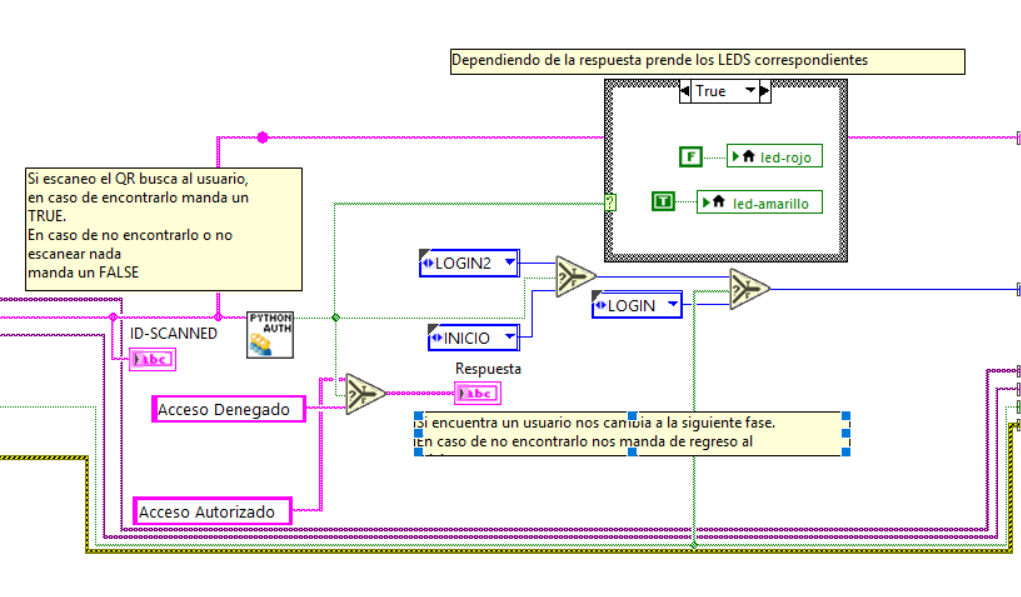
\includegraphics{images/title-page/lb-con5.png}};

        \node[anchor=center,scale=.9,text width=8cm,xshift=2cm,yshift=0cm,align=justify] (tx8) at (im10.north){
            Despues de escanear el QR\dots
        };
    \end{tikzpicture}
\end{frame}

\subsection{Programa en LabVIEW pt.4}

\begin{frame}[t]{Interfaz en LabVIEW}{Diagrama de flujo pt.4}
    \begin{tikzpicture}[remember picture,overlay]

        \node[anchor=center,scale=.9,text width=8cm,xshift=0cm,yshift=3cm,align=center] (tx10) at (current page.center){
            Si la persona pasa el 1er filtro\dots
        };

        \node[anchor=center,scale=.4,xshift=0cm,yshift=-8.5cm](im11) at (tx10.south){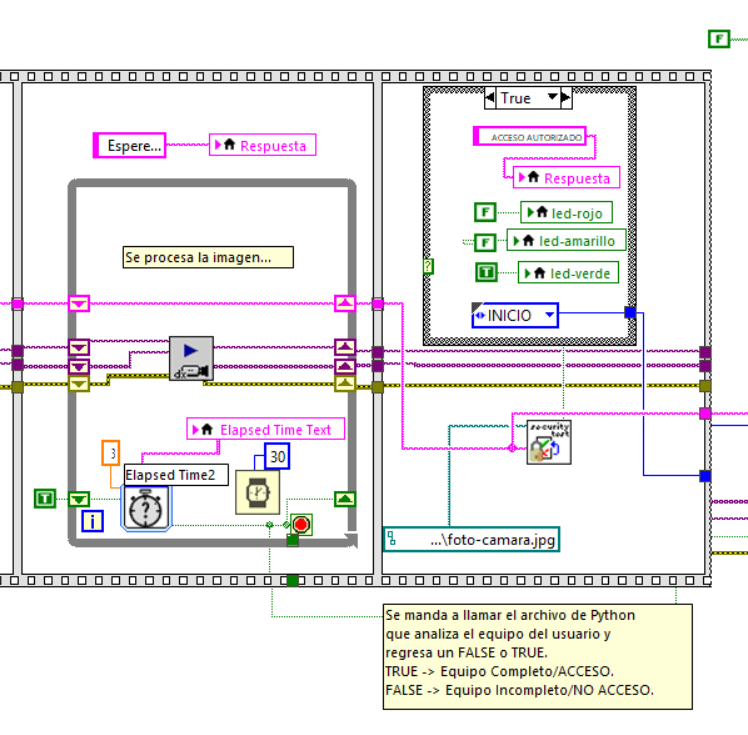
\includegraphics{images/title-page/lb-con7.png}};
    \end{tikzpicture}
\end{frame}

\subsection{Funciones adicionales}

\begin{frame}[t]{LabVIEW}{Funciones Extra [Gestión de usuarios]}
    \begin{tikzpicture}[remember picture,overlay]
        \node[anchor=center,scale=.9,text width=8cm,xshift=4cm,yshift=3cm,align=center] (tx11) at (current page.west){
            Función para agregar usuario\dots
        };

        \node[anchor=center,scale=.4,xshift=0cm,yshift=-7cm] (im12) at (tx11.south){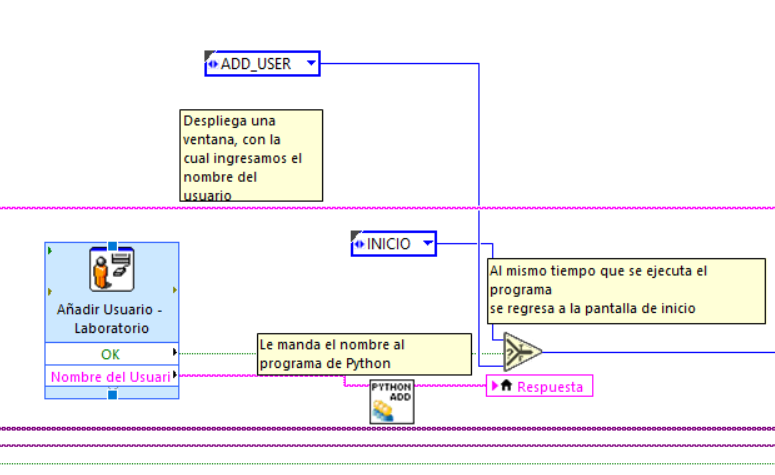
\includegraphics{images/title-page/lb-con8.png}};

        \node[anchor=center,scale=.9,text width=8cm,xshift=-6cm,yshift=3cm,align=center] (tx12) at (current page.east){
            Función para eliminar usuario\dots
        };

        \node[anchor=center,scale=.4,xshift=0cm,yshift=-7cm] (im13) at (tx12.south){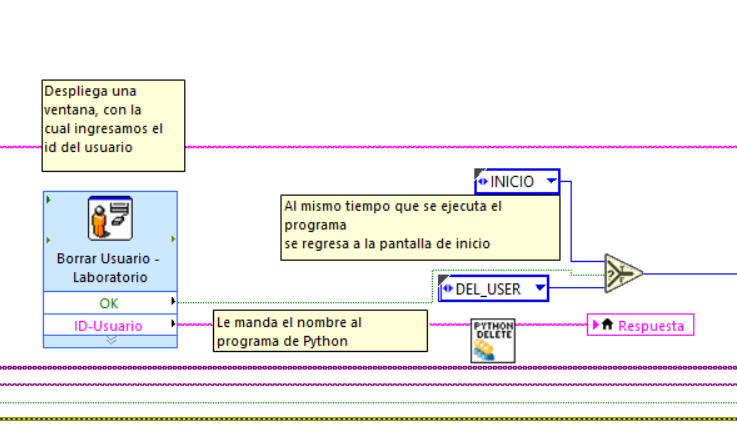
\includegraphics{images/title-page/lb-con9.png}};
    \end{tikzpicture}
\end{frame}

\subsection{Panel Frontal}

\begin{frame}[t]{Panel Frontal}{Interacción del Usuario}
    \begin{tikzpicture}
        \node[anchor=center,scale=.9,text width=16cm,xshift=0cm,yshift=3cm,align=center] (tx13) at (current page.center){
            Como resultado, nuestro panel frontal es el siguiente:
        };

        \node[anchor=center,scale=.32,xshift=0cm,yshift=-10cm,align=center] (im14) at (tx13.south){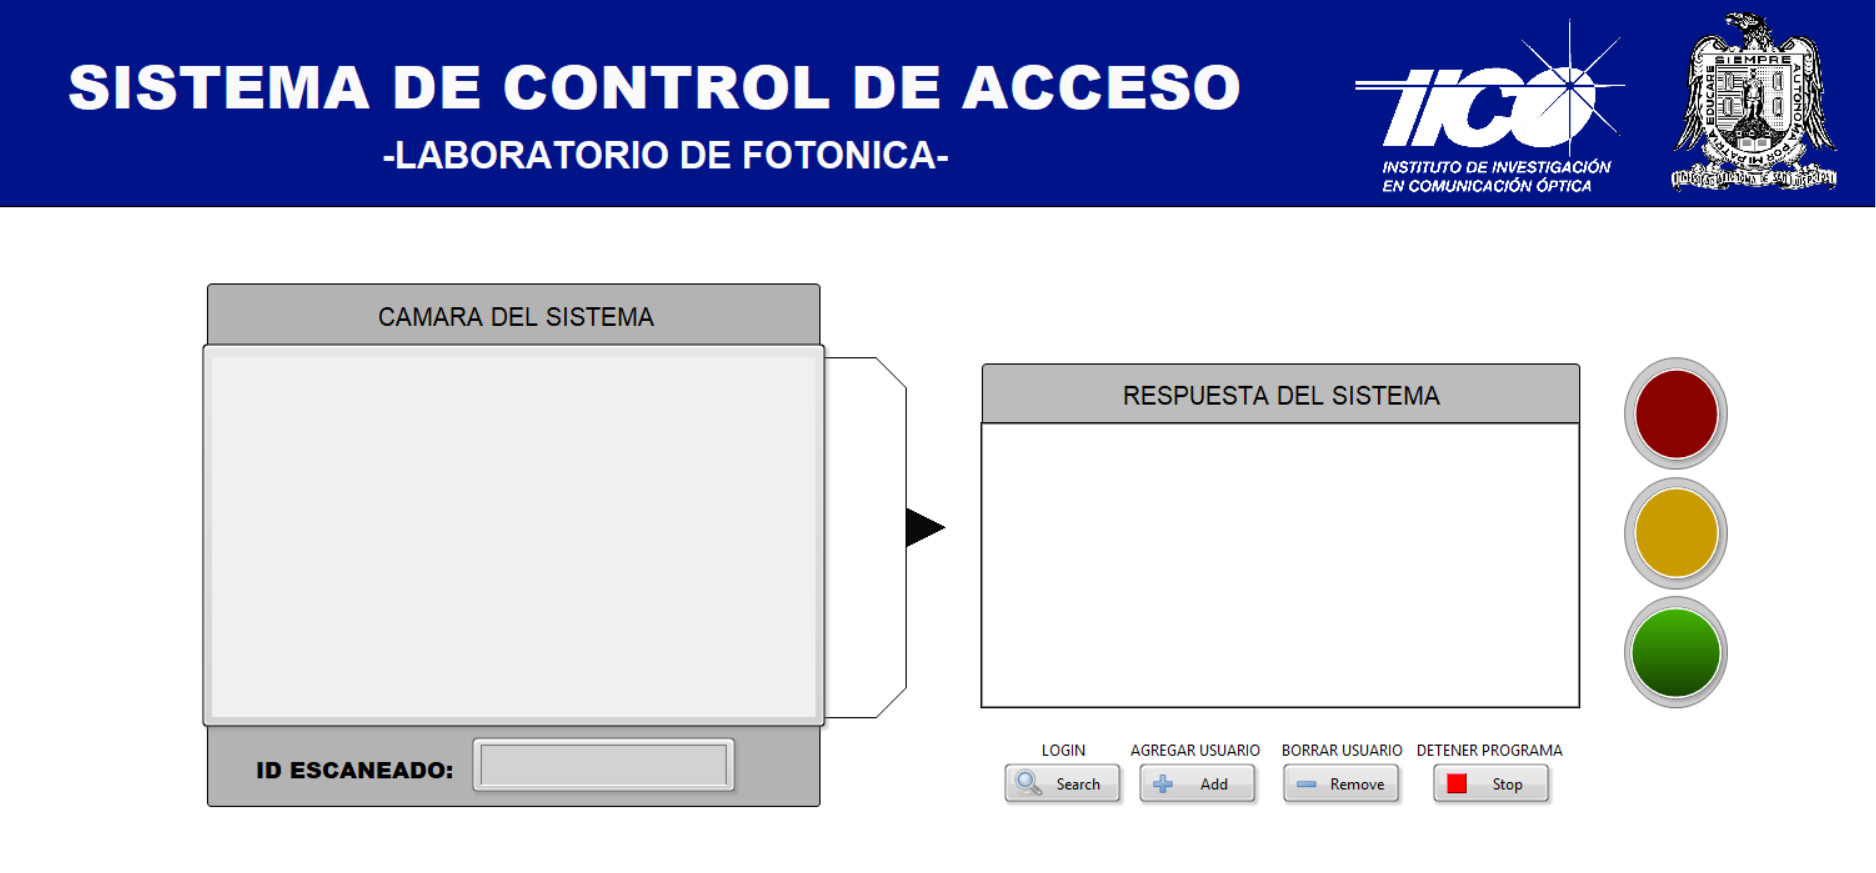
\includegraphics{images/title-page/lb-con10.png}};
    \end{tikzpicture}
\end{frame}


\section{Conclusiones}

\begin{frame}[t]{Final}{hemo acabao mi gente}
    \begin{tikzpicture}[remember picture,overlay]
        \node[anchor=center,scale=.9,xshift=0cm,yshift=0cm,align=justify,text width=16cm]at (current page.center){
            Se lograron los siguientes resultados:
            \begin{itemize}
                \item implementación de APIs para sistema funcional de monitoreo de seguridad por medio de Python.
                \item Conexión Python - LabVIEW para agilizar el manejo de datos.
                \item Sistema no dependiente de Python ya que LabVIEW realiza su trabajo independientemente de lo que haga Python.
            \end{itemize}
        };
    \end{tikzpicture}
\end{frame}

\section{Agradecimientos}

\begin{frame}[t]{Gracias}{Gracias Gracias Gracias}
    \begin{tikzpicture}[remember picture,overlay]

        \node[anchor=center,scale=.9,xshift=0cm,yshift=-.5cm] at (current page.center){
\includegraphics{images/title-page/fin2.jpg}};
        
    \end{tikzpicture}
\end{frame}

\end{document}